

\tikzset{every picture/.style={line width=0.75pt}} %set default line width to 0.75pt        

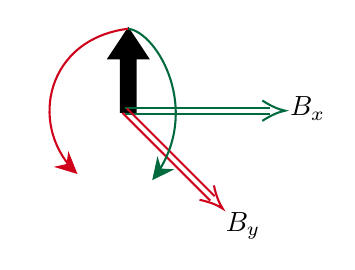
\begin{tikzpicture}[x=0.75pt,y=0.75pt,yscale=-1,xscale=1]
%uncomment if require: \path (0,300); %set diagram left start at 0, and has height of 300

%Up Arrow [id:dp8569712747307681] 
\draw  [fill={rgb, 255:red, 0; green, 0; blue, 0 }  ,fill opacity=1 ] (79,75.33) -- (88.5,61) -- (98,75.33) -- (92.03,75.33) -- (92.03,101) -- (84.97,101) -- (84.97,75.33) -- cycle ;
%Straight Lines [id:da365595300658881] 
\draw [color={rgb, 255:red, 0; green, 105; blue, 62 }  ,draw opacity=1 ]   (86.8,98.99) -- (157,98.99)(86.8,101.99) -- (157,101.99) ;
\draw [shift={(164,100.49)}, rotate = 180] [color={rgb, 255:red, 0; green, 105; blue, 62 }  ,draw opacity=1 ][line width=0.75]    (10.93,-4.9) .. controls (6.95,-2.3) and (3.31,-0.67) .. (0,0) .. controls (3.31,0.67) and (6.95,2.3) .. (10.93,4.9)   ;
%Straight Lines [id:da16660066105443272] 
\draw [color={rgb, 255:red, 208; green, 2; blue, 27 }  ,draw opacity=1 ]   (87.86,99.43) -- (130.11,141.68)(85.74,101.55) -- (127.99,143.8) ;
\draw [shift={(134,147.69)}, rotate = 225] [color={rgb, 255:red, 208; green, 2; blue, 27 }  ,draw opacity=1 ][line width=0.75]    (10.93,-4.9) .. controls (6.95,-2.3) and (3.31,-0.67) .. (0,0) .. controls (3.31,0.67) and (6.95,2.3) .. (10.93,4.9)   ;
%Curve Lines [id:da30971168582376674] 
\draw [color={rgb, 255:red, 208; green, 2; blue, 27 }  ,draw opacity=1 ]   (88.5,61) .. controls (49.21,65.85) and (40.51,106.45) .. (61.93,128.96) ;
\draw [shift={(64,131)}, rotate = 222.51] [fill={rgb, 255:red, 208; green, 2; blue, 27 }  ,fill opacity=1 ][line width=0.08]  [draw opacity=0] (10.72,-5.15) -- (0,0) -- (10.72,5.15) -- (7.12,0) -- cycle    ;
%Curve Lines [id:da25524324543733845] 
\draw [color={rgb, 255:red, 0; green, 105; blue, 62 }  ,draw opacity=1 ]   (88.5,61) .. controls (102.71,62.96) and (124.12,100.45) .. (101.44,132.07) ;
\draw [shift={(100,134)}, rotate = 308] [fill={rgb, 255:red, 0; green, 105; blue, 62 }  ,fill opacity=1 ][line width=0.08]  [draw opacity=0] (10.72,-5.15) -- (0,0) -- (10.72,5.15) -- (7.12,0) -- cycle    ;

% Text Node
\draw (165,92.4) node [anchor=north west][inner sep=0.75pt]    {$B_{x}$};
% Text Node
\draw (134,148.09) node [anchor=north west][inner sep=0.75pt]    {$B_{y}$};


\end{tikzpicture}
